\documentclass[a4paper,12pt]{report}

% Page layout
\usepackage[left=2.5cm,right=2.5cm,top=2.5cm,bottom=2.5cm]{geometry}

% Font and text
\usepackage[afrikaans,english]{babel}
\usepackage{microtype}
\usepackage{setspace}
\usepackage{lmodern}
\usepackage{siunitx}
\newcommand{\myemph}[1]{{\sffamily\bfseries#1}}
\sloppy
\onehalfspacing

% Headings
\usepackage[raggedright,sf,bf]{titlesec}
\usepackage[margin=\the\parindent,small,bf,sf]{caption}
\titlelabel{\thetitle.\ }
\titleformat{\chapter}[display]{\huge\bfseries\sffamily}{\chaptertitlename\ \thechapter}{15pt}{\Huge \raggedright}
\titlespacing*{\chapter}{0pt}{0pt}{40pt}  % remove spacing before chapter headings
\makeatletter
\let\originall@chapter\l@chapter
\def\l@chapter#1#2{\originall@chapter{{\sffamily #1}}{#2}}
\makeatother

%% Alternative headings using small-caps (comment out the top section)
%\usepackage[raggedright,bf]{titlesec}
%\usepackage[margin=\the\parindent,small,bf]{caption}
%\titlelabel{\thetitle.\ }
%\titleformat{\chapter}[display]{\huge\scshape}{\chaptertitlename\ \thechapter}{15pt}{\Huge \raggedright}
%\titlespacing*{\chapter}{0pt}{0pt}{40pt}  % remove spacing before chapter headings

% Table of contents
\let \savenumberline \numberline
\def \numberline#1{\savenumberline{#1.}}

% Figures
\usepackage{graphicx}
\usepackage{pdfpages}
\usepackage{subcaption}
\setlength{\abovecaptionskip}{7.5pt}  % spacing above and below captions
\newcommand*{\WaterMark}[2][0.2\paperwidth]{\AddToShipoutPicture*{\AtTextCenter{\parbox[c]{0pt}{\makebox[0pt][c]{\includegraphics[width=#1]{#2}}}}}}

% Mathematics
\usepackage[cmex10]{amsmath}
\usepackage{amssymb}
\usepackage{cancel}
\DeclareMathOperator*{\argmax}{arg\,max}
\newcommand{\T}{^\top}
\newcommand{\tr}{\textrm{tr}}
\renewcommand{\vec}[1]{\boldsymbol{\mathbf{#1}}}
\newcommand{\defeq}{\triangleq}

% Tables
\usepackage{booktabs}
\usepackage{tabularx}
\usepackage{multirow}
\newcommand{\mytable}{
    \centering
    \small
    \renewcommand{\arraystretch}{1.2}
    }
\renewcommand{\tabularxcolumn}[1]{m{#1}}
\newcolumntype{C}{>{\centering\arraybackslash}X}
\newcolumntype{L}{>{\raggedright\arraybackslash}X}

% Header and footer
\usepackage{fancyhdr}
\pagestyle{fancy}
\fancyhf{}
\renewcommand{\sectionmark}[1]{\markright{\normalsize \thesection.\ #1}}
\fancyhead[C]{\nouppercase{\textit{\rightmark}}}
\fancyhead[RO]{\thepage}
 \fancyhead[LE]{\thepage}  % double-sided printing
\fancyfoot{}
\setlength\headheight{14.5pt}
\renewcommand{\headrulewidth}{0pt}
\fancypagestyle{plain}{\fancyhead{}
                       \renewcommand{\headrulewidth}{0pt}
                       \fancyfoot[C]{\thepage}}

% Pseudo-code
\usepackage{algorithm}  % should go before \usepackage{hyperref}

% Table of contents and hyperlinks
\usepackage{hyperref}
\hypersetup{colorlinks=true,linktoc=all,citecolor=black,linkcolor=black}
\usepackage[nottoc]{tocbibind}

% Pseudo-code
\usepackage{algpseudocode}  % should go after \usepackage{hyperref}
\renewcommand{\thealgorithm}{\arabic{chapter}.\arabic{algorithm}} 
\captionsetup[algorithm]{labelfont={bf,sf},font=small,labelsep=colon}

% Bibliography
\usepackage{cite}  % automatically reorder inline citations
\bibliographystyle{IEEEtran}

% Fix titlesec issue
\usepackage{etoolbox}
\makeatletter
\patchcmd{\ttlh@hang}{\parindent\z@}{\parindent\z@\leavevmode}{}{}
\patchcmd{\ttlh@hang}{\noindent}{}{}{}
\makeatother


\begin{document}

% Front matter
\graphicspath{{frontmatter/fig/}}
\pagenumbering{Alph}

\begin{titlepage}
	\begin{center}
		
		
\includegraphics[width=10cm]{USlogo-top}
		
		\vfill
		
		{\sffamily \bfseries \huge Foot strike pattern determination with a battery-powered device and Android application. \par}
%		{\scshape \huge A Critical Analysis of Design Flaws in the Death Star \par}
		
		\vfill
		
		{\large {\Large Dewaldt Snyman} \\ 22706852 \par}
		
		\vfill
		
		\vfill
		
		{Report submitted in partial fulfilment of the requirements of the module \\
			Project (E) 448 for the degree Baccalaureus in Engineering in the Department of
			Electrical and Electronic Engineering at Stellenbosch University. \par}
		
		\vfill
		
		{\large {Supervisor}: Dr W.\ A.\ Smit} %\\
		% Department of Electrical and Electronic Engineering \par}
		
		\vfill
		
		{\Large 31 October 2022}
	\end{center}
\end{titlepage}

%\graphicspath{{frontmatter/fig/}}
\pagenumbering{Alph}

\begin{titlepage}
	\begin{center}
		
		%
\includegraphics[width=10cm]{USlogo-top}
		
		\WaterMark{UScrest-WM}
		
		~\vspace{4.5em}
		
		{\sffamily \bfseries \huge A Critical Analysis of Design Flaws in the Death Star \par}
%		{\scshape \huge A Critical Analysis of Design Flaws in the Death Star \par}		
		
		\vspace{7em}
		
		{\large {\Large  Luke Skywalker} \\ 99652154 \par}
		
		\vspace{8em}
		
		{\large Thesis presented in partial fulfilment of the requirements for the degree of \\ Master of Engineering (Electronic) in the Faculty of Engineering at Stellenbosch University. \par}
		
		\vfill
		
		{\large {Supervisor}: Dr O.\ W.\ Kenobi\\
		Department of Electrical and Electronic Engineering \par}
		
		%\vfill
		\vspace{10em}
		
		{\Large October 2099}
	\end{center}
\end{titlepage}

\pagenumbering{roman}
\chapter*{Acknowledgements}
% \addcontentsline{toc}{chapter}{Acknowledgements}
\makeatletter\@mkboth{}{Acknowledgements}\makeatother

I would like to thank my family and friends for all the support without them all of this would not have been possible. Finally, I would like to thank Dr Willem Smit, my skirpsie coordinator, for all the advice and support with this skripsie.
%\chapter*{Declaration}
\newpage
\thispagestyle{plain}
\addcontentsline{toc}{chapter}{Declaration}
\makeatletter\@mkboth{}{Declaration}\makeatother

\centerline{
\includegraphics[width=8cm]{USlogo-top}}
\vspace*{-10pt}

\section*{\centering Plagiaatverklaring / \textit{Plagiarism Declaration}}

\vspace*{5pt}

\begin{enumerate}
    \item Plagiaat is die oorneem en gebruik van die idees, materiaal en ander intellektuele eiendom van ander persone asof dit jou eie werk is.\\
    \textit{Plagiarism is the use of ideas, material and other intellectual property of another's work
        and to present is as my own.}
    
    \item Ek erken dat die pleeg van plagiaat 'n strafbare oortreding is aangesien dit 'n vorm van diefstal is.\\
    \textit{I agree that plagiarism is a punishable offence because it constitutes theft.}
    
    \item Ek verstaan ook dat direkte vertalings plagiaat is. \\
    \textit{I also understand that direct translations are plagiarism.}
    
    \item Dienooreenkomstig is alle aanhalings en bydraes vanuit enige bron (ingesluit die internet) volledig verwys (erken). Ek erken dat die woordelikse aanhaal van teks sonder aanhalingstekens (selfs al word die bron volledig erken) plagiaat is. \\
    \textit{Accordingly all quotations and contributions from any source whatsoever (including the internet) have been cited fully. I understand that the reproduction of text without quotation marks (even when the source is cited) is plagiarism}
    
    \item Ek verklaar dat die werk in hierdie skryfstuk vervat, behalwe waar anders aangedui, my eie oorspronklike werk is en dat ek dit nie vantevore in die geheel of gedeeltelik ingehandig het vir bepunting in hierdie module/werkstuk of 'n ander module/werkstuk~nie. \\
    \textit{I declare that the work contained in this assignment, except where otherwise stated, is my original work and that I have not previously (in its entirety or in part) submitted it for grading in this module/assignment or another module/assignment.}
\end{enumerate}

\vfill

\noindent \begin{tabularx}{1.0\linewidth}{|L|L|}
    \hline
    \vspace{1cm} {Studentenommer / \textit{Student number}} & \vspace{1cm} {Handtekening / \textit{Signature}} \\
    \hline
    \vspace{1cm} {Voorletters en van / \textit{Initials and surname}} & \vspace{1cm} {Datum / \textit{Date}} \\
    \hline
\end{tabularx}

\vspace{15pt}

% The old declaration

%I, the undersigned, hereby declare that the work contained in this report is my own original work unless otherwise stated.
%
%% Afrikaans:
%% Hiermee verklaar ek, die ondergetekende, dat die werk in hierdie verslag vervat my eie oorspronklike werk is, tensy anders vermeld.
%
%\vspace{2.5cm}
%
%\begin{table}[h]
%\begin{tabular}{@{}p{2.5cm}p{5cm}}
%    Signature: & \dotfill \\
%    & \multicolumn{1}{c}{Obi-Wan Kenobi} \\
%    ~\vspace{1cm} \\
%    Date: & \dotfill \\
%\end{tabular}
%\end{table}
%
%\vfill
%
%\begin{center}
%    Copyright \textcopyright\ 2099 Stellenbosch University \\
%    All rights reserved
%\end{center}


\chapter*{Abstract}
\addcontentsline{toc}{chapter}{Abstract}
\makeatletter\@mkboth{}{Abstract}\makeatother

\subsubsection*{English}

\selectlanguage{english}
This document is a technical report on the design and development of a mobile application capable of using data readings from a prototype pressure-sensing footwear device to display foot strike patterns and other relevant information. This information could help with health analysis, like the gait analysis, on runners and other athletes. This application could be a tool for healthcare professionals and high-performance athletes.

The prototype device can continuously sample ADC measurements from a portable device with 8 FSR cells. This FSR device fits in the sole of a shoe, and ADC measurements from the FSR device are read and transmitted by the Arduino. The transmission happens via BLE (Bluetooth Low Energy). The Android application can then connect to the Arduino, receive these ADC readings, and use the data to display the foot strike patterns of a user. The foot strike patterns are displayed on a heatmap using the power of openGL|ES. The force exerted on each cell can be calculated by calibrating each cell and using the necessary mathematics to formulate a graph that relates the force to the ADC values. The prototype device has battery power and fits in a casing that allows users to strap the device to their legs.

A new casing was designed and printed with a 3D printer to cover the prototype device circuitry.
\clearpage
\subsubsection*{Afrikaans}
\selectlanguage{afrikaans}

Hierdie dokument is 'n tegniese verslag oor die ontwerp en ontwikkeling van 'n mobiele toepassing wat datalesings van 'n prototipe drukwaarnemende skoentoestel kan neem om voetstakingpatrone en ander relevante inligting te vertoon. Hierdie inligting kan help met gesondheidsanalises, soos die Gait analise, op hardlopers en ander atlete. Hierdie toepassing kan 'n hulpmiddel wees vir afrigters en atlete.


Die prototipe toestel kan voortdurend analoog na digitale lesings neem vanaf 'n draagbare toestel met 8 drukkrag sensitiewe resistor selle. Hierdie Ftoestel pas in die sool van 'n skoen, en analoog na digitale word deur die Arduino opgeneem en oorgedra. Die oordrag vind plaas via BLE (Bluetooth Low Energy). Die Android-toepassing kan dan aan die Arduino koppel, hierdie ADC-lesings ontvang en die data gebruik om die voetstakingpatrone van 'n gebruiker te vertoon. Die voetstakingpatrone word op 'n hittekaart(heatmap) vertoon met behulp van die krag van openGL|ES. Die drukkrag wat op elke sel uitgeoefen word, kan bereken word deur elke sel te kalibreer en die nodige wiskunde te gebruik om 'n grafiek te formuleer wat die krag met die analog na digitale waardes in verband bring. Die prototipe toestel het batterykrag en pas in 'n omhulsel waarmee gebruikers die toestel aan hul bene kan vasbind.

'N Nuwe omhulsel is ontwerp en gedruk met 'n 3D -drukker om die stroombaan van die prototipe toestel te bedek.


\tableofcontents
\listoffigures
\listoftables
\chapter*{Nomenclature\markboth{}{Nomenclature}}
\addcontentsline{toc}{chapter}{Nomenclature}

% \vspace*{-3mm}
% \subsubsection*{Variables and functions}

% \begingroup
% \renewcommand{\arraystretch}{1.2}
% \renewcommand{\tabularxcolumn}[1]{p{#1}}
% \begin{tabularx}{\textwidth}{@{}p{2.5cm}L}
%     $p(x)$ & Probability density function with respect to variable $x$.\\
%     $P(A)$ & Probability of event $A$ occurring.\\
%     $\varepsilon$ & The Bayes error. \\
%     $\varepsilon_u$ & The Bhattacharyya bound. \\
%     $B$ & The Bhattacharyya distance. \\
%     $s$ & An HMM state.  A subscript is used to refer to a particular state, e.g.\ $s_i$ refers to the $i^{\text{th}}$ state of an HMM. \\
%     $\mathbf{S}$ & A set of HMM states. \\
%     $\mathbf{F}$ & A set of frames. \\
%     $\mathbf{o}_f$ & Observation (feature) vector associated with frame $f$. \\
%     $\gamma_s(\mathbf{o}_f)$ & A posteriori probability of the observation vector $\mathbf{o}_f$ being generated by HMM state $s$. \\
%     $\mu$ & Statistical mean vector. \\
%     $\Sigma$ & Statistical covariance matrix. \\
%     $L(\mathbf{S})$ & Log likelihood of the set of HMM states $\mathbf{S}$ generating the training set observation vectors assigned to the states in that set. \\
%     $\mathcal{N}(\mathbf{x} | \mu, \Sigma)$ & Multivariate Gaussian PDF with mean $\mu$ and covariance matrix $\Sigma$.\\
%     $a_{ij}$ & The probability of a transition from HMM state $s_i$ to state $s_j$. \\
%     $N$ & Total number of frames or number of tokens, depending on the context. \\
%     $D$ & Number of deletion errors. \\
%     $I$ & Number of insertion errors. \\
%     $S$ & Number of substitution errors. \\
% \end{tabularx}
% \endgroup


% \newpage
\subsection*{Acronyms and abbreviations}

\begingroup
\renewcommand{\arraystretch}{1.2}
\begin{tabular}{@{}p{2.5cm} l}
    % AE      & Afrikaans English \\
    % AID     & accent identification \\
    % ASR     & automatic speech recognition \\
    % AST     & African Speech Technology \\
    % CE      & Cape Flats English \\
    % DCD     & dialect-context-dependent \\
    % DNN		& deep neural network \\
    % G2P     & grapheme-to-phoneme \\
    % GMM     & Gaussian mixture model \\
    % HMM     & hidden Markov model \\
    % HTK     & Hidden Markov Model Toolkit \\
    % IE      & Indian South African English \\
    % IPA     & International Phonetic Alphabet \\
    % LM      & language model \\
    % LMS     & language model scaling factor \\
    % MFCC    & Mel-frequency cepstral coefficient \\
    % MLLR    & maximum likelihood linear regression \\
    % OOV     & out-of-vocabulary \\
    % PD      & pronunciation dictionary \\
    % PDF     & probability density function \\
    % SAE     & South African English \\
    % SAMPA   & Speech Assessment Methods Phonetic Alphabet \\
    FSR     & Force Sensing Resistor\\
    MCU     & Micro Controller Unit\\
    BLE     & Bluetooth Low Energy\\

\end{tabular}
\endgroup

\newpage
\pagenumbering{arabic}

% Contents
\graphicspath{{introduction/fig/}}

\chapter{Introduction}
\label{chap:introduction}


In the modern day, jogging is one of the most popular physical activities. People all over the world partake in this physical activity. One would think that jogging is a simple exercise and there are no major injury or health concerns. However, there are some major concerns as jogging has a high injury rate. Over the past few years, there has been an increasing interest in this subject and many studies have been conducted on how these injuries can be analyzed. Strike patterns during running has been acknowledged as potential way of identifying injuries or risk of injury. 





\section{Problem Statement}
Develop an application that can use data from a prototype device and display the foot strike patterns from this data. Do additional calculations to show the ground force applied with each step. The raw data should be processed and saved to be displayed and used in useful manners such as videos and graphs. 
\section{Objectives}
% TODO: this sucks
The objective of this project is to use a prototype wearable device that captures the pressure applied to a grid of pressure sensing resistors. The prototype has been build by a previous student and is capable of capturing the data from FSR cells and transmitting the data via BLE. An mobile application should then be developed to receive this data, process it and display or save it in useful ways.The application can then be used by medical experts to assist in medical assessments like the Gait analysis. 
\section{Scope and Limitations}

The scope of this project is to only design and develop an andriod application that displays the foot strike patterns captured by the prototype device. As the device was built by a predecessor there are some design flaws that had to be considered:
\begin{itemize}
    \item Very large device
    \item The Arduino used does not have enough ADC channels and an extra component was added taking up more space. 
    \item The battery of the device is very large and adds a large amount of weights to a device that should be wearable.
    \item The charging circuit is not in working order and the battery had to be manually charged.
  \end{itemize}

\section{Overview of the report}

Chapter 2 Lit review

Chapter 3 System design

Chapter 4 Detailed design

Chapter 5 Tests

Chapter 6 Summary conclusions


\section{Section heading}

This is some section with two table in it: Table~\ref{tbl:exemplars} and Table~\ref{tbl:abx_speaker}.

\begin{table}[!h]
    \mytable
    \caption{Performance of the unconstrained segmental Bayesian model on TIDigits1 over iterations in which the reference set is refined.}
    \begin{tabularx}{\linewidth}{@{}lCCCCC@{}}
        \toprule
        Metric     & 1 & 2 & 3 & 4 & 5 \\
        \midrule
        WER (\%)                        & $35.4$ & $23.5$ & $21.5$ & $21.2$ & $22.9$ \\
        Average cluster purity (\%)       & $86.5$ & $89.7$ & $89.2$ & $88.5$ & $86.6$ \\
        Word boundary $F$-score (\%)         & $70.6$ & $72.2$ & $71.8$ & $70.9$ & $69.4$ \\
        Clusters covering 90\% of data   & 20             & 13 & 13 & 13 & 13 \\
        \bottomrule
    \end{tabularx}
    \label{tbl:exemplars}
\end{table}


\begin{table}[!h]
    \renewcommand{\arraystretch}{1.1}
    \centering
    \caption{A table with an example of using multiple columns.}
    \begin{tabularx}{0.65\linewidth}{@{}lCCr@{}}
        \toprule
        & \multicolumn{2}{c}{Accuracy (\%)} \\
        \cmidrule(lr){2-3}
        Model    & Intermediate & Output & Bitrate\\
        \midrule
        Baseline & 27.5         & 26.4   & 116 \\
        VQ-VAE   & 26.0         & 22.1   & 190 \\
        CatVAE   & 28.7         & 24.3   & 215 \\
        \bottomrule
    \end{tabularx}
    \label{tbl:abx_speaker}
\end{table}

\newpage

This is a new page, showing what the page headings looks like, and showing how to refer to a figure like Figure~\ref{fig:cae_siamese}.

\begin{figure}[!t]
    \centering
%     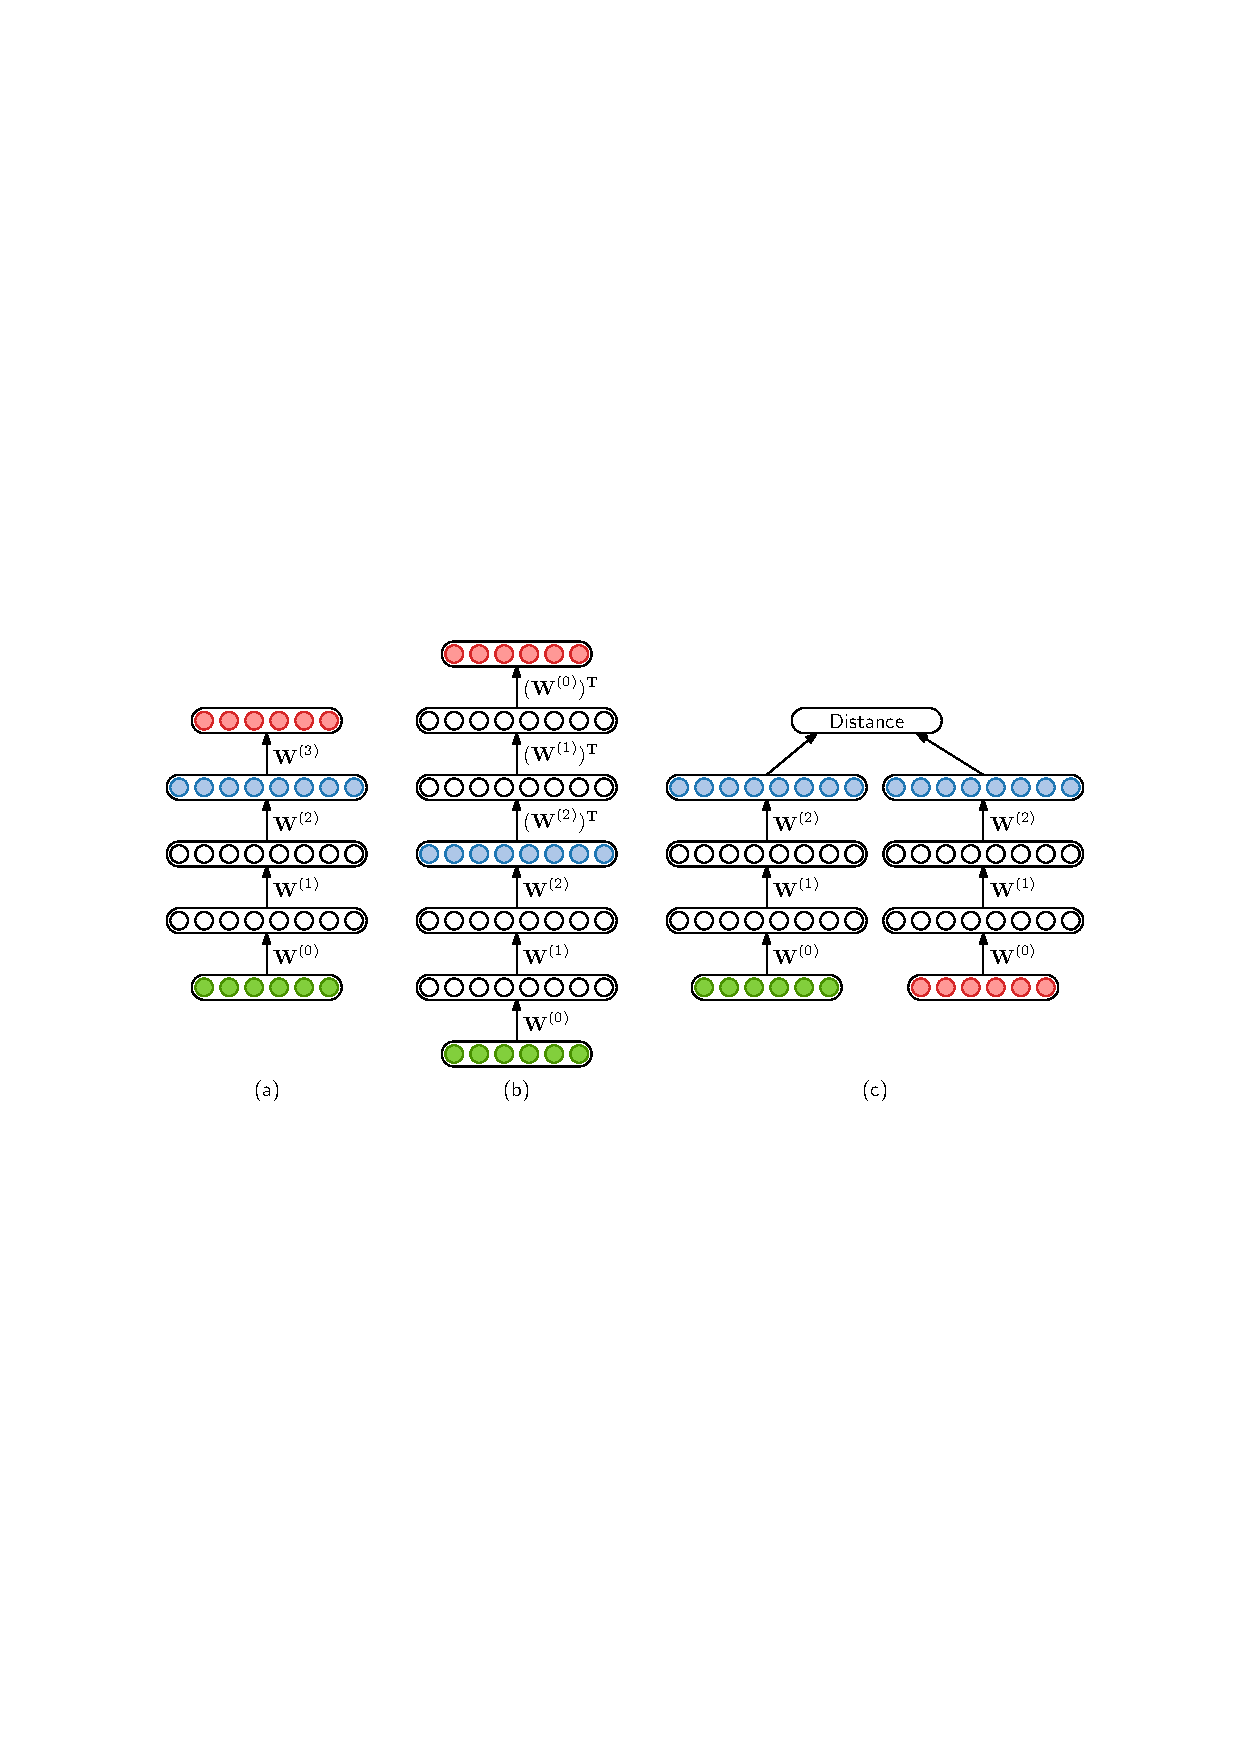
\includegraphics[width=\linewidth]{cae_siamese}
    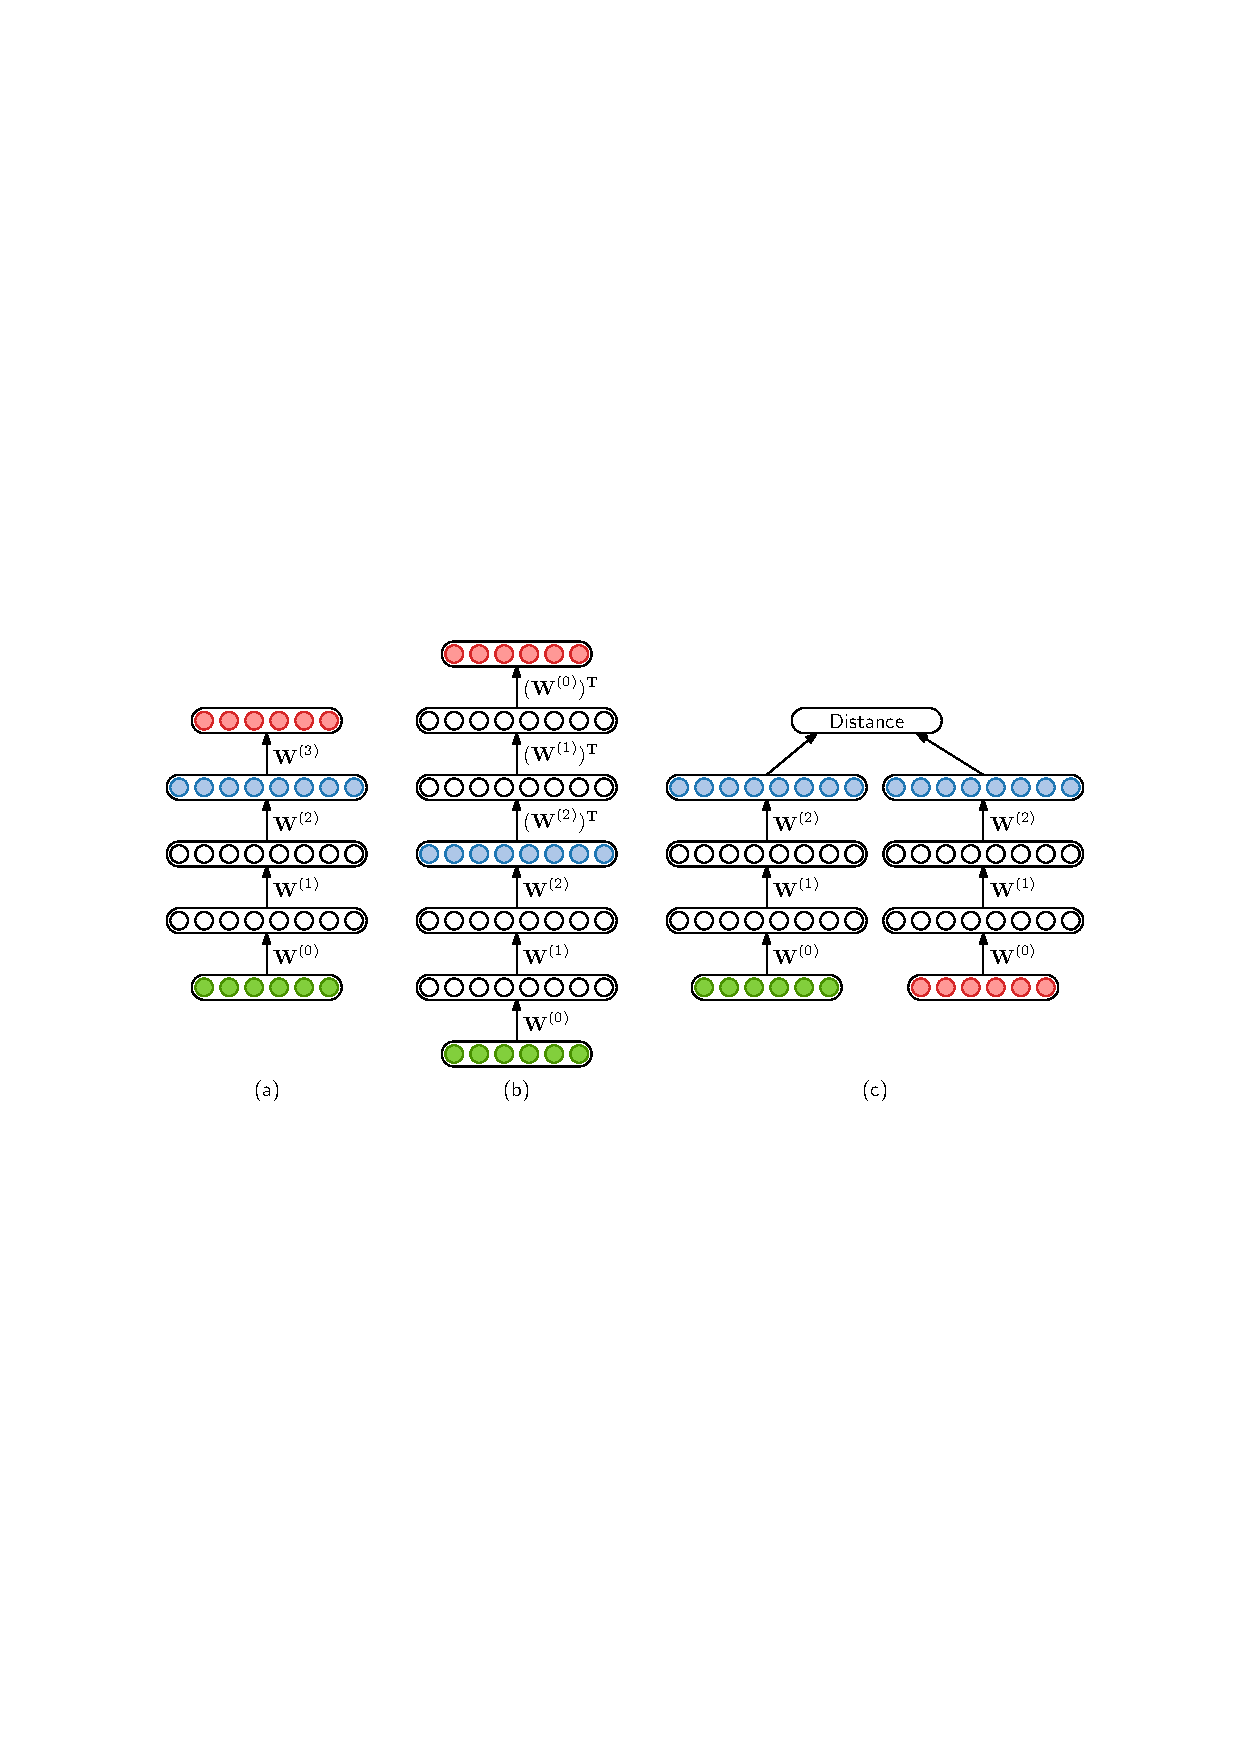
\includegraphics[width=0.918\linewidth]{cae_siamese}
    \caption[I am the short caption that appears in the list of figures, without references.]{
    (a) The cAE as used in this chapter. The encoding layer (blue) is chosen based on performance on a development set.
    (b) The cAE with symmetrical tied weights. The encoding from the middle layer (blue) is always used.
    (c) The siamese DNN. The cosine distance between aligned frames (green and red) is either minimized or maximized depending on whether the frames belong to the same (discovered) word or not.
    A cAE can be seen as a type of DNN~\cite{dahl+etal_taslp12}.
    }
    \label{fig:cae_siamese}
\end{figure}


The following is an example of an equation:
\begin{equation}
P(\vec{z} | \vec{\alpha}) = \int_{\vec{\pi}} P(\vec{z} | \vec{\pi}) \, p(\vec{\pi} | \vec{\alpha}) \, \textrm{d} \vec{\pi}
= \int_{\vec{\pi}} \prod_{k = 1}^K \pi_k^{N_k} \frac{1}{B(\vec{\alpha})} \prod_{k = 1}^K \pi_k^{\alpha_k - 1} \, \textrm{d} \vec{\pi}
\label{eq:example_equation}
\end{equation}
which you can subsequently refer to as~\eqref{eq:example_equation} or Equation~\ref{eq:example_equation}.
But make sure to consistently use the one or the other (and not mix the two ways of referring to equations).
\graphicspath{{litreview/fig/}}

\chapter{Literature Review}
\label{chap:litreview}
\section{Foot strike patterns and Gait analysis}
\label{sec:Gait}
Running is a popular everyday physical activity worldwide, and statistics prove this\cite{statistaresearchdepartment2020}. Although running is a simple activity, it involves complex movements and integrating muscles, joints, and various body parts. These complex movements cause running to be a common physical activity that typically causes injuries. In-depth studies on foot strike patterns elsewhere \cite{doi:10.2519/jospt.2015.6019}, \cite{CAVANAGH1980397
}, \cite{matheuso.almeidaptphdirenes.davisptphdalexandred.lopesptphd2015}, \cite{lauram.andersondanielr.bonannoharvif.hart&christianj.barton2020} review the basics of foot strike patterns and the biomechanics of running. These in-depth studies are beyond the scope of this technical report, but these reviews provide relevant information to understand better what causes these injuries. These studies indicate that considering foot motion during walking and running is crucial to understanding why running can commonly lead to injuries. It has been proven in studies such as \cite{kennethp.clarklaurencej.ryanpeterg.weyand2014} that running performance, energy requirements, and musculoskeletal stresses are directly related to foot strike patterns and action-reaction force between the limb and the ground. 

Factors like foot strike patterns, footwear conditions, running speed, and environmental conditions can affect a human's biomechanics during running. According to \cite{matheuso.almeidaptphdirenes.davisptphdalexandred.lopesptphd2015} there are three primary foot strike patterns: forefoot, rearfoot (heel strike), and midfoot. Forefoot striking is when the anterior region of the foot strikes the ground first. Midfoot striking is when the posterior and anterior parts of the foot hit the ground simultaneously, and rearfoot or heel strike is when the heel or rear area of the foot strikes the ground initially. According to \cite{marEfootstrike} \cite{matheuso.almeidaptphdirenes.davisptphdalexandred.lopesptphd2015} majority of both mid-distance and long-distance runners are heel strikers. This would explain why running shoes are heavily padded at the heel part of the shoe. This padding makes the landing process more comfortable. See Figure \ref{fig:footstrike} for an excellent visual representation of the different strikes. There are many benefits of knowing one's foot strike patterns. For instance, specialists use foot strike patterns in the Gait analysis.
\clearpage
\begin{figure}[!htb]
    \centering
    \includegraphics[width = 0.7\linewidth]{Screenshot 2022-10-11 153343.png}
    \caption{Image found in an online article\cite{mass4d2017} illustrating the Foot Strike Patterns in Runners.}
    \label{fig:footstrike}
\end{figure}

Gait analysis studies human motion using observer instruments to measure body movement, body mechanics, and muscle activity. Gait analysis is commonly used in biomechanics to help athletes prevent or recover from injuries. The gait analysis identifies posture- or movement-related problems that can cause injuries. Identifying these problems allows professionals to advise and train athletes to move more efficiently in their sport, mainly when running or walking. Foot pressures are regularly used in the systematic physical examination of athletes, such as the Gait analysis \cite{Baker2006}. Further reading shows that foot strike patterns, step rate, and posture can be combined for gait modifications and to reduce the impact of the load on body parts during running. The study \cite{HUANG2019102} from the Journal of Biomechanics demonstrates this with a series of experiments where runners were analyzed as seen in figure \ref{fig:examplegait}  

\begin{figure}[!htb]
    \centering
    \includegraphics[width = 0.7\linewidth]{examplegait.jpg}
    \caption{Example of how gait analysis can be for runners}
    \label{fig:examplegait}
\end{figure}


\newpage
\section{Technology used for Gait analysis}
\label{technologygair}

\begin{table}[!h]
    \mytable
    \caption{Summary of running gait parameters that different sensors and systems can measure  \cite{higginsonbrian2009}.}
    \begin{tabularx}{\linewidth}{@{}lC@{}}
        \toprule
        Sensor\textbackslash System     & Measurements and outcomes \\
        \midrule
        Motion analysis systems                       & Linear and angular velocity, and acceleration. The body orientation and positioning.\\
        Force platforms    & Ground reaction force and joint moment. This system can measure power by using motion analysis along with force platforms. \\
        Pressure sensors        & Pressure distribution of the foot. Vertical force, the center of pressure, and spatiotemporal measurements. \\
        Electromyography  & Muscle activation and muscle fatigue.\\
        Accelerometers  & Acceleration and orientation.n\\
        Electrogoniometers  & Relative joint angles.\\
        Gyroscopes  & Orientation, angular velocity, and acceleration.\\
        \bottomrule
    \end{tabularx}
    \label{tbl:exemplars}
\end{table}
\clearpage
\section{Bluetooth Low Energy BLE}
\label{sec:ble}

\subsection{How Does BLE Work?}
\label{sec:howdoesblework}

When using Bluetooth Low Energy, it is essential to know the roles of each device. These roles are defined by the Generic Attribute Profile(GATT).In all BLE applications, there are two roles: the \textbf{central} and the \textbf{peripheral} devices. \cite{josebagur2022} The peripheral device will be the device that broadcasts or advertises information, and the central device will be scanning for information. A good visual representation of how BLE works is to think of an advertising board where the peripheral device keeps pinning new info onto the board, and the central device scans the board and uses the information available. These two devices have unique addresses. The peripheral will be advertising information to nearby devices, while the central device will look for any devices that advertise information; when the central device finds the advertised information, it attempts to connect to the peripheral device. Once a connection is established, the central device can start reading or writing information from or to the peripheral device.

\begin{figure}[!h]
    \centering
    \includegraphics[width = 0.6\linewidth]{BLE.png}
    \caption{Basic BLE overview}
    \label{fig:bleoverview}
\end{figure}



\subsection{Services, Characteristics Descriptor and Properties}
\label{sec:servicesandcharacteristics}
The GATT structure for BLE can be explained in the following hierarchical order. A service is a collection of characteristics; each characteristic has properties and a descriptor that describes the characteristic. See the basic illustration below \ref{fig:ble_roles}.

\begin{figure}[!h]
    \centering
    \includegraphics[width = 0.5\linewidth]{blehierarchy.png}
    \caption{Basic hierarchy of GATT structure for BLE}
    \label{fig:ble_roles}
\end{figure}

Each \textbf{service} has its unique identifying code called a UUID. The UUID allows one peripheral device to have multiple services and can be 128-bit long for each service. A service can also be seen as a group of capabilities. For example, a smartwatch can measure heart rate and temperature and track GPS location. These three capabilities can be grouped under one service called the activity service. This method of grouping information allows the central device to understand the information that the peripheral is advertising.

The capabilities mentioned in the above example are better known as \textbf{characteristics}. Each characteristic has its unique identifying code called, also known as a UUID, which allows one service to have multiple characteristics. A characteristic can be seen as a single capability. For example, the heart rate measurement is one characteristic. This characteristic can be seen as a single capability of the activity service. 

A characteristic has other attributes that help describe the value that it contains. These attributes are \textbf{properties} and \textbf{descriptors}. Properties describe how the characteristic can be used. Properties represent several bits that indicate whether the characteristic is set to read, write, write without response, notify or indicate. The descriptor contains information about the characteristic value and how it should be interpreted. The descriptor can be user descriptions, format, and units of the value or extended properties of the value\cite{mohammadafaneh2017}. For example, the heart rate characteristic can be a range of the heart rate measurement, and the descriptor defines this range.


\section{Force Sensitive Resistors}
A Force Sensitive Resistor (FSR) is a piezoresistive electrical component, meaning a change in the electrical resistivity can be detected when mechanical strain is applied. Most FSR devices specify that they can measure force at temperatures as high as 200$^\circ C$. FSRs consists of three layers: a semi-conductive material/semi-conductive ink between two substrates. There are two types of FSRs: Shunt Mode and Thru Mode.

Shunt mode FSRs have polymer thick-film layers that have two separate parts. These parts are separated with a spacer. The shunt mode FSR is the most common and basic type of FSR and is also used by the IEEE foot sensor. This type of FSR would change resistance when pressure is applied, and the ink touches the electrodes. The more pressure applied more ink touches the electrodes and yields the voltage change across the resistor.

Thru Mode FSRs are made of polyester film layers which are positioned on the outer parts, while a conductive silver circle with traces secures the pressure-sensitive layers. An adhesive layer will then laminate the two layers together. See \ref{fig:fsr} for a graphical illustration of the two types of FSRs. Figure \ref{fig:fsr}, along with more tutorials on the use of FSRs, was found here \cite{tekscan2022}, \cite{gigiseeedstudio2020}

\begin{figure}[!h]
    \centering
    \includegraphics[width = 0.7\linewidth]{fsr.jpg}
    \caption{An illustration of the two types of FSRs and their different layers.}
    \label{fig:fsr}
\end{figure}

% A FSR typically consists of 3 layers; a top resistive polymer layer, a thin bottom
% film polymer layer with conductive traces and a middle spacer layer separating the top
% and bottom layers. The three layers are often enclosed in a flexible polymer.
% When there is no pressure applied the top resistive layer and bottom conductive layer
% are completely separated by the spacer and act as an open circuit (infinite resistor).
% As pressure is applied to the FSR the top resistive layer is pressed against the bottom
% conductive layer causing the resistance to decrease.

\section{Open GLES for android}
\label{sec:OpenGL}
OpenGL is an open-source graphics library for high-performance 2D and 3D graphics rendering. OpenGL|ES is a flavor of OpenGL intended explicitly for embedded and mobile devices. OpenGL|ES is a cross-platform, high-performance graphics API that Android devices can use. Android supports the framework API and the Native Development Kit (NDK) of OpenGL.  

\begin{figure}[!h]
    \centering
    \includegraphics[width = 0.9\linewidth]{pipeline.png}
    \caption{OpenGl pipeline diagram adapted from \cite{androidmakersbenjaminmonjoie2017}}
    \label{fig:openglpipeline}
\end{figure}
The primary pipeline of OpenGL and also OpenGLES starts by defining vertices. These are the points to draw a shape in a 2D or 3D space. These raw vertices are passed to the vertex shader to be processed. The vertex shader code will give these points a position on the screen. Next, the processed vertices are passed to the rasterizer. The rasterizer describes a virtual scene. The best way to understand this is to look at the visual explanation in figure \ref{fig:rasterizer  }. The geometry of what is to be displayed is described with vertices. The rasterizer projects this geometry onto a 2D plane, which is the screen. The vertices are called fragments after they have been projected. These fragments are mapped with textures or colors by the fragment shader, depending on what is to be displayed. After that, all the fragments are merged to represent the final output to the display. All this information is compiled from the video presetion\cite{media.ccc.defolkert2019} by folkert. Here he explains all the basics, mathematics, and code of OpenGL.
\clearpage
\begin{figure}[]
    \includegraphics[width = 0.9\linewidth]{Rasterizer.png}
    \caption{Rasterizer illustration}
    \label{fig:rasterizer}
\end{figure}

Regarding the Android framework, two foundational classes allow manipulating graphics with OpenGL ES API. These two classes are $GLSurfaceView$ and $GLSurfaceView.Renderer$. It is best to understand the implementation of these two classes to use OpenGL in an Android application.\cite{androiddevelopers2022}\\
\\
\textbf{GLSurfaceView}\\
This class is a View that can draw and control objects utilizing OpenGL API. This class is very similar to the $SurfaceView$ in functionality. To use the $GLSurfaceView$ class, create an instance of it and add a renderer. It is also possible to extend this class to allow for touchscreen functionality.
\\
\textbf{GLSurfaceView.Renderer}\\
This interface needs to be implemented as a separate class. This class should then be attached to the $GLSurfaceView$ class by using $GLSurfaceView.setRenderer()$. This interface defines the methods required for drawing. These methods are the following:
\begin{itemize}
    \item onSurfaceCreated(): This method is called when the GLSurfaceView is created. This method contains the actions needed to set up and initialize all the parameters and objects that are needed for an OpenGL ES environment. This method will only be called once.
    \item onDrawFrame(): This method is called each time, and a graphics object is drawn and redrawn. 
    \item onSurfaceChanged(): This method is called when the system finds that the geometry has changed. The geometry can change when the orientation of the device screen is changed, like changing from portrait to landscape, or when the size of the $GLSurfaceView$ changes.
\end{itemize}
\graphicspath{{conclusion/fig/}}

\chapter{Summary and Conclusion}
\label{chap:conclusion}
An Android application displaying foot strike patterns was successfully designed, developed, and tested. The final application has the following features:
\begin{itemize}
    \item Bluetooth connection to specific Arduino device
    \item Heatmap that displays the data from the foot sensor
    \item Table that displays the calculated force and force distribution
    \item Ability to record video and comma-delimited data in CSV format. Both files are saved on the user's phone.
    \item Option to load previously recorded data and play it on the application
  \end{itemize}

The application also had a feature that calculated the user's steps, but there was no use for this in the current state of the application. Not having two devices made it difficult to calculate the user's total steps for both feet. This feature will be added to further work to, for example, calculate cadence.

  It was possible to conduct some tests using the device and application features. Some observations could be made, like seeing less pressure on the FSR cells when walking on grass than on a hard surface. It was also seen how walking uphill differs from walking downhill and what type of foot strike patterns all the tests yields. Another interesting observation was that the shoes used for testing had slightly lifted heels, influencing the strike patterns as the heel FSR cells received more pressure when standing in a mid-stance position.

  Video recordings demonstrating the features of the device and application were shown to the staff of the Sports Science Faculty, and there was much interest in the device and application. The primary concern was the device, which indicates what is to be done in further work. The link to the videos mentioned follows. The following link is an example video of walking uphill \cite{dewaldtsnymanup2022}, and this link \cite{dewaldtsnymandown2022} is an example video of walking downhill. 

  Some functionality could not be achieved due to time constraints and limitations. This is mainly because only one prototype device was available, and the prototype device had design choices that constrained the development of possible features.


\clearpage
\chapter{Further Work}
\label{chap:furtherwork}

\section{Device}

As mentioned in section \ref{limitations} the current prototype does have some limitations. These limitations include that it is difficult to duplicate this device, and the weight and geometry of the device do not allow it to be used for running. The Arduino Nano 33 BLE also lacks the necessary analog pins. Therefore a re-design is recommended for the prototype device. A device like the ESP32 would better fit a prototype device. The ESP32 has a sufficient amount of analog pins, and some models have built-in charging circuits making it easier to build multiple copies of the possible design.

As mentioned in section \ref{technologygair} other sensors could be used for further analysis. The Arduino Nano 33 BLE has an accelerometer and gyroscope that are not used in the project's current state. These types of sensors should be considered when designing a new prototype device.

Another recommendation is to re-calibrate or refactor the foot sensor device. There are companies like Stappone\cite{stappone}  who have much more sophisticated devices. This indicates that it is possible to build a better sensor device.
\section{Application}

Lastly,  exploring the capabilities of OpneGLES would allow for more advanced 3D rendered images or even live 3D movements, as this is all well in the capabilities of OpenGLES.
If a new prototype device allows it, the application can have further functionality like:
\begin{itemize}
    \item Cadence
    \item Strike length
    \item Power
    \item Speed and acceleration 
  \end{itemize}


% Bibliography
\bibliography{mybib}

% End matter
\appendix
\graphicspath{{appendices/fig/}}
\chapter{Project Planning Schedule}
\makeatletter\@mkboth{}{Appendix}\makeatother
\label{appen:projectplan}
    \begin{tabular}{ | m{5em} |c|m{12cm}| }
      \hline
      \textbf{Date} & \textbf{Week} & \textbf{Description} \\
      \hline
      Jul 18-23 & 1 & Project planning and scope \\ 
      \hline
      25-30 & 2 & Study prototype devices and how it can be used.\\ 
      \hline
      Aug 01-6 & 3 & Literature study on the topic at hand. This is everything that is correlated to running and foot strike patterns \\ 
      \hline
      8-13 and 15-20 & 4 and 5 & Start developing the Arduino code for the device. Try to get basic ADC readings from the IEEE foot sensor The previous student could not provide previously written code. \\ 
      \hline
      22-27 & 6 & Reach BLE and how it can be used to transmit data from an Arduino device. Start developing the code as soon as I have good understanding of BLE for Arduino \\ 
      \hline
      Aug 29 - Sept 3& 7 & Test Week \\ 
      \hline
      5-10 & 8 & Recess \\ 
      \hline
      12-17 and 19-24  & 9 and 10 & Start building the Android application and understand BLE regarding Android devices. Display the data transmitted from the Arduino in a text view \\ 
      \hline
      26- 1 Oct and 3-8 & 11 and 12 & Build a heatmap view using OpenGL|ES. This requires a good understanding of OpenGL|ES and custom Android views  \\ 
      \hline
      10-15 & 13 & Use the previous students calibrations to build another custom view that displays the force exerted in newton on each cell \\ 
      \hline
      17-22  & 14 & Test the application. This includes using the device on difference surfaces and walking up or down a hill. See if temperature has an effect on the cell readings \\ 
      \hline
      24-29 & 15 & Present application to a person who has knowledge of foot strike patterns to see if an application of such would be of use in the industry and reflect on findings \\ 
      \hline
      31 October 2022 & 16 & Report Deadline. Prepare for oral examination \\ 
      \hline
    \end{tabular}
\chapter{Outcomes Compliance}
\makeatletter\@mkboth{}{Appendix}\makeatother
\label{appen:derivations_bigramseg}

\begin{center}.
  \begin{tabular}{ | m{4cm} |c|m{10cm}| }
    \hline
    \textbf{ELO} & \textbf{Chapter} & \textbf{Description} \\
    \hline
    1. Problem solving & 1,2,3,4 & Chapter 1 demonstrates the identification and formulation of an engineering problem.
    
    Chapter 2 and 3 demonstrates the analysis of the problem and previous solutions
    
    Chapter 4 demonstrates how the problem was solved by developing an android application\\ 
    \hline
    2. Application of scientific and engineering knowledge & 3,4,5 & Chapter 3 and 4 demonstrates the use of mathematics and engineering fundamentals to design and program an application that can do advance calculations.\\ 
    \hline
    3. Engineering Design & 3,4 & Chapter 3 demonstrates the understanding of engineering design. Chapter 4 demonstrates the design and synthesis of and engineering idea by developing Arduino and Java code.   \\ 
    \hline
    4. Investigations, experiments and data analysis & 5 & Chapter5 demonstrates the investigations of different ways to test the device an application. The data could be retrieved from the various tests and the data was analyzed. \\ 
    \hline
    5. Engineering methods, skills, and tools, including Information Technology & 4,Appendix C & Chapter 4 demonstrates the use of programming skills in C++ and Java. In Chapter 4 mathematical tools such as Desmos was used. Appendix C demonstrates the design and print of a 3D model using ZBrush\\ 
    \hline
    6. Professional and technical communications& 6 & Chapter 6 demonstrates that the device an application were demonstrated to people in the field of sports science. Their feedback can be used for future work and recommendations. \\ 
    \hline
    7. Individual Work & All & The whole of the project was conducted individually \\ 
    \hline
    8. Independent learning ability& 2,4 & Chapter 2 demonstrates the ability to learn new concepts and skills and chapter 4 demonstrates how these newly found concepts and skills were implemented.\\
    \hline
  \end{tabular}
  \end{center}

\chapter{3D Model of device casing}
\makeatletter\@mkboth{}{Appendix}\makeatother
\label{appen:3dmodel}

\begin{figure}[!htb]
  \centering
  \includegraphics[width = 1\linewidth]{ortos_1.jpg}
  \caption{Top shell 3D model}
  \label{fig:CustomTableLayout}
\end{figure}

\begin{figure}[!htb]
  \centering
  \includegraphics[width = 1\linewidth]{ortos_2.jpg}
  \caption{Base 3D model}
  \label{fig:CustomTableLayout}
\end{figure}

\begin{figure}[!htb]
  \centering
  \includegraphics[width = 1\linewidth]{ortos_complete.jpg}
  \caption{Assembled base and shell}
  \label{fig:CustomTableLayout}
\end{figure}

\chapter{Prototype Device}
\makeatletter\@mkboth{}{Appendix}\makeatother
\label{appen:prototype}

\begin{figure}[!htb]
  \centering
  \includegraphics[width = 0.7\linewidth]{device3.jpg}
  \caption{Prototype device without the foot sensor connected}
  \label{fig:CustomTableLayout}
\end{figure}

\begin{figure}[!htb]
  \centering
  \includegraphics[width = 0.7\linewidth]{device1.jpg}
  \caption{Prototype device with the foot sensor connected}
  \label{fig:CustomTableLayout}
\end{figure}

\begin{figure}[!htb]
  \centering
  \includegraphics[width = 0.7\linewidth]{device2.jpg}
  \caption{Prototype device fitted in a casing with the foot sensor connected}
  \label{fig:CustomTableLayout}
\end{figure}

\chapter{Android Application}
\makeatletter\@mkboth{}{Appendix}\makeatother
\label{appen:androidapp}

\begin{figure}[!htb]
  \centering
  \includegraphics[width = 0.5\linewidth]{demo1.jpg}
  \caption{Main Screen with all the features}
  \label{fig:CustomTableLayout}
\end{figure}

\begin{figure}[!htb]
  \centering
  \includegraphics[width = 0.5\linewidth]{demo2.jpg}
  \caption{File picker pop-up}
  \label{fig:CustomTableLayout}
\end{figure}

\begin{figure}[!htb]
  \centering
  \includegraphics[width = 0.5\linewidth]{demo3.jpg}
  \caption{Enter file name pop-up}
  \label{fig:CustomTableLayout}
\end{figure}

\chapter{Smart Footwear Sensing Solutions by IEE}
\makeatletter\@mkboth{}{Appendix}\makeatother
\label{appen:footweardevice}

\begin{figure}[!htb]
  \centering
  \includegraphics[width = 0.7\linewidth]{footsensor.png}
  \caption{IEE foot sensor specifications and labeling for each cell}
  \label{fig:footsensordevice}
\end{figure}


\end{document}

